%%%%%%%%%%%%%%%%%%%%%%%%%%%%%%%%%%%%%%%%%%%%%%%%%%%%%%%
% Math 3250 Combinatorics, University of Connecticut
%%%%%%%%%%%%%%%%%%%%%%%%%%%%%%%%%%%%%%%%%%%%%%%%%%%%%%%

% Anything after a percent sign is a comment.

% Necessary first line. \documentclass defines the type of document and some options (for example, try changing the font size (10pt or 11pt or 12pt).
\documentclass[10pt]{amsart}
\usepackage{enumerate} % to be able to enumerate a list using non-numbers
\usepackage{tikz}
%for hypertext references
\usepackage[colorlinks = true,
            linkcolor = blue,
            urlcolor  = blue,
            citecolor = red,
            anchorcolor = green]{hyperref}


\usepackage[letterpaper]{geometry} 
\geometry{tmargin=0.3in,bmargin=0.0in,lmargin=0.50in,rmargin=0.50in}
\voffset -0.6in

% The part of the tex file between the \documentclass and \begin{document} line is called the preamble.  Things having to do with setting up the document are done in the preamble.  You will not need to mess with it for now, except to change your name and the title of your document. 
% After adding your name next to author, head down to where it says "Start here"

\title{Math3250 Combinatorics Reading HW 14}
%\author{your preferred first and last name:}
%\date{}
\begin{document}

\maketitle

% --------------------------------------------------------
%                         Start here
% --------------------------------------------------------

%\noindent Credit: 
%Write down everyone who helped you, including classmates who contributed to your thought process. Write down Bona's textbook and other written sources you used as well.

\subsection*{Instruction}

\begin{itemize}
\item Do all sections.
Submit your homework by email (subject: Math3250 Combinatorics Reading HW 14). Either type or hand-write your work (use a scanner app to convert to PDF)
\item
Ref: textbook \emph{Combinatorics and Graph Theory} by Harris, Hirst, and Mossinghoff (HHM) Sec 1.2 and 
 B\'ona's ``A Walk through Combinatorics" textbook, Chapter 9
\end{itemize}






\section{Watch or read: HHM Sec 1.2  Distance in graphs}

Do one of the following:
\begin{enumerate}[i.]
	\item Finish watching \href{}{lecture video of Sec 1.2 Distance of graphs} 
	\item Finish reading only the parts highlighted in color  \href{https://egunawan.github.io/combinatorics/notes/notes1_2distance_in_graphs.pdf}{lecture notes for Sec 1.2 video}
\end{enumerate}

Write down what you did. If you watched the video, please specify (Kaltura/YouTube) and type of device.


\section{Exercises (complete all)}



Write down the definition of \emph{adjacency matrix} and \emph{distance matrix}. 
Give the adjacency matrix and the distance matrix of each of the following families of graphs:

\begin{enumerate}[a.)]
\item
the path graph $P_{n}$, 
where the vertices are labeled from one end of the path to the other.

\begin{center}
	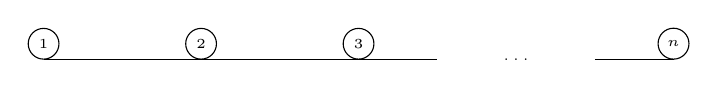
\begin{tikzpicture}[scale=2]
	\tiny
	\node [draw, circle,above] at (1,0) {$1$};
	\node [draw, circle,above] at (2,0) {$2$};
	\node [draw, circle,above] at (3,0) {$3$};
	\node at (4,0) {$\dots$};
	\node [draw, circle,above] at (5,0) {$n$};
	\draw (1,0) -- (2,0) -- (3,0) -- (3.5,0) (4.5,0)--(5,0);
	\end{tikzpicture}
\end{center}

\item 
the cycle graph $C_{2k}$ and $C_{2k+1}$, where the vertices are labeled consecutively around the cycle, \textit{e.g.} 

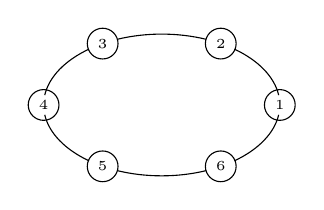
\begin{tikzpicture}[xscale=0.5, yscale=0.3]
\tiny
\def \n {6}
\def \radius {3cm}
\def \margin {8} % margin in angles, depends on the radius

\foreach \s in {1,...,\n}
{
	\node[draw, circle] at ({360/\n * (\s - 1)}:\radius) {$\s$};
	\draw[] ({360/\n * (\s - 1)+\margin}:\radius) 
	arc ({360/\n * (\s - 1)+\margin}:{360/\n * (\s)-\margin}:\radius);
}
\end{tikzpicture}
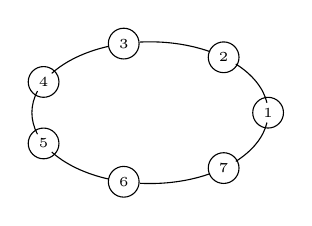
\begin{tikzpicture}[xscale=0.5, yscale=0.3]
\tiny
\def \n {7}
\def \radius {3cm}
\def \margin {8} % margin in angles, depends on the radius

\foreach \s in {1,...,\n}
{
	\node[draw, circle] at ({360/\n * (\s - 1)}:\radius) {$\s$};
	\draw[] ({360/\n * (\s - 1)+\margin}:\radius) 
	arc ({360/\n * (\s - 1)+\margin}:{360/\n * (\s)-\margin}:\radius);
}
\end{tikzpicture}

\item 
the complete bipartite graph $K_{m,n}$, where the vertices in the first partite set are labeled $1,2,\dots,m$.
\item  
the complete graph $K_{n}$, any labeling.
\\

\item 
Without computing the matrix directly, find $A^3$ where $A$ is the adjacency matrix of the complete graph $K_4$ (shown below). Use Theorem 1.7 in HHM. Recall that 
$
\tiny
A=
\begin{bmatrix}
	0 & 1 & 1 & 1\\
	1 & 0 & 1 & 1\\
	1 & 1 & 0 & 1\\
	1 & 1 & 1 & 0
\end{bmatrix}
$
since there is an edge between every pair of vertices. 


\begin{center}
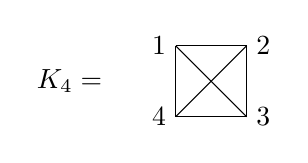
\begin{tikzpicture}[scale=0.9]
\draw (0,0) -- (1,0);
\draw (0,1) -- (1,1);
\draw (0,0) -- (0,1);
\draw (1,0) -- (1,1);
\draw (0,0) -- (1,1);
\draw (1,0) -- (0,1);
\draw (0,1) node[left] {$1$};
\draw (0,0) node[left] {$4$};
\draw (1,1) node[right] {$2$};
\draw (1,0) node[right] {$3$};
\draw (-1.5,0.5) node {$K_4=$};
\end{tikzpicture}
\end{center}



\item 
If $A$ is the adjacency matrix for a graph $G$, show that the $(j,j)$ entry of $A^2$ is the degree of $v_j$. (Previously there was a typo.)
\\

\item 
Find the ordinary generating function for the number of edges of the complete graph $K_n$, $n\geq 1$.

\item Find the exponential generating function for the number of edges of the complete graph $K_n$, $n\geq 1$.


\end{enumerate}








\section{Presentations}
\begin{itemize}
	\item Pick several exercises (of out the eight listed above), and prepare to explain them during class meeting.
	\item Make sure to tell me your preferences ahead of time (to save time)
\end{itemize}

%It's fine (and maybe better for you) if you pick questions that you don't feel 100\% about.




\section{Last Section}

Do one of the following:
\begin{enumerate}
\item
Read about 1/2 of the blog post
\href{https://www.math3ma.com/blog/matrices-probability-graphs}{math3ma.com/blog/matrices-probability-graphs} by 
T.-D.~Bradley 
which explains how every $m \times n$ matrix corresponds to a weighted bipartite graph, and matrix multiplication is the same as gluing two graphs and traveling along paths. 
Then
mimic 
the graph-gluing process that the author did for matrix multiplication $MN$, but for the following matrices:

$
\tiny
M=
\begin{bmatrix}
1 & 2 & 3\\
0 & -2 & 4
\end{bmatrix},
N = 
\begin{bmatrix}
5 \\
0 \\
-1
\end{bmatrix}.
$

\item
Read \emph{one} of the following four passages from HHM Sec 1.2.3 (p. 26--30): Acquaintance Graph / Hollywood Graph/ Mathematical Collaboration graph / Small World Networks. Then briefly summarize the main idea.


\end{enumerate}


%\section{Comments}
%\begin{enumerate}[i.]  
%\item Approximately how much time did you spend on this homework (including reading or watching the videos)?
%%\item You are encouraged to communicate with your classmates. Write down the resources (for example, a textbook or a  \href{https://math.stackexchange.com/}{math.stackexchange.com/} page) you referenced and the people that you talked with.	
%\item 
%What can I do to improve your remote learning experience? 
%Questions or other comments?
%\end{enumerate}




\end{document}
